% =====================================================================
%  CLAIMARC -- Experiments and Conclusion (Sections 4-5)
%  Compile with: xelatex claimarc_paper.tex  (needs xeCJK + Songti SC)
%  Figures in ./figs (PDF).
% =====================================================================
\documentclass[11pt]{article}
\usepackage[margin=1in]{geometry}
\usepackage{amsmath,amssymb}
\usepackage{graphicx}
\usepackage{booktabs}
\usepackage{multirow}
\usepackage{array}
\usepackage{xcolor}
\usepackage{caption}
\usepackage[hidelinks]{hyperref}
\usepackage{fontspec}
\usepackage{xeCJK}
\setCJKmainfont{Songti SC}
\captionsetup{font=small,labelfont=bf}
\setlength{\parskip}{2pt}
\newcommand{\best}[1]{\textbf{#1}}
\newcommand{\std}[1]{{\scriptsize$\pm$#1}}

\title{\vspace{-2em}From Objective Verification to Consumer Perception:\\
A Retrieval-Augmented Contrastive Framework for Misleading-Advertising\\
Detection in Livestream E-Commerce\\[0.4em]
\large (Experiments and Conclusion)}
\author{}
\date{}

\begin{document}
\maketitle
\vspace{-3em}

\setcounter{section}{3}

\section{Experiments}
\label{sec:exp}

Our empirical study is organized around four research questions.
\textbf{RQ1} asks whether CLAIMARC discriminates perceived-misleading
advertising more accurately than the three baseline families, namely
objective fact verification, single-stream text classification, and large
language models. \textbf{RQ2} asks whether retrieval-augmented contrastive
learning (RACL) shapes a representation that tightens same-label claim--evidence
pairs and separates pairs carrying opposite perceived-risk labels.
\textbf{RQ3} asks whether the trained model transfers to unseen categories and
streamers, and whether a frozen-encoder retrieval library can absorb new domains
without parameter re-training. \textbf{RQ4} asks which components, retrieval
choices, and hyper-parameters drive the result. Section~\ref{sec:exp:main}
answers RQ1; Section~\ref{sec:exp:xdom} answers RQ3;
Section~\ref{sec:exp:geom} answers RQ2; and
Sections~\ref{sec:exp:abl}--\ref{sec:exp:select} answer RQ4 and characterize
the deployment behavior of the model.

\subsection{Data and Descriptive Statistics}
\label{sec:exp:data}

The corpus covers Chinese livestream e-commerce sessions collected between
October 2024 and March 2025. After the \S3.2.1 pipeline (per-category
attribute normalization, streamer-claim alignment, and three-source
product-fact extraction), each instance is a $(\text{product},
\text{attribute})$ pair, written $(p,a)$. Two kinds of pairs enter the data.
Comment-driven pairs receive a perceived-risk label from aligned consumer
comments. Objective-negative pairs cover attributes a streamer asserted but
for which no consumer comment aligned; these carry no perceived-misleading
signal ($y{=}0$) and are weighted by the coverage of product-side evidence.
The final dataset contains \best{4{,}883} pairs spanning \best{10} first-level
categories, \best{38} sub-categories, \best{108} livestream rooms, and
\best{1{,}532} normalized attributes, of which 2{,}278 are comment-driven and
2{,}605 are objective-negative. The positive (misleading) class accounts for
\best{25.6\%} of the pairs, so the task is a class-imbalanced screening
problem rather than a balanced classification one.

We partition the data 70:10:20 by \texttt{room\_id}, keeping every pair of a
room inside a single split so that no streamer appears in both training and
test. Table~\ref{tab:data} reports the partition. The three splits hold
positive rates of 24.2\%, 31.1\%, and 29.1\%, which are close enough to treat
the test distribution as representative. Evidence-source coverage, counting how
many of the three product-fact sources fire for a pair, is distributed as
1{,}483 / 1{,}826 / 1{,}118 / 456 pairs for 0 / 1 / 2 / 3 sources (mean 1.11),
and the instance-level reliability weight $c_{p,a}$ has mean 0.456, median
0.48, and a bulk in $[0.18, 0.82]$. A streamer-claim segment runs about 23
characters and a product-fact text about 22 characters. Among all pairs,
46.7\% align to at least one relevant consumer comment, with 6.9 aligned
comments per pair on average and 1.5 of them negative; these aligned comments
form the empirical basis of the perceived-risk label. The category counts in
Table~\ref{tab:cat} are long-tailed, led by apparel, baby-and-kids, and a
general bucket, and this tail is what the cross-category transfer study in
Section~\ref{sec:exp:xdom} stresses.

\begin{table}[t]
\centering\small
\setlength{\tabcolsep}{8pt}
\begin{tabular}{lrrr}
\toprule
\textbf{Split} & \textbf{\#Pairs} & \textbf{Pos.\ \%} & \textbf{\#Rooms} \\
\midrule
Train & 3{,}636 & 24.2 & 92 \\
Val   & 392     & 31.1 & 5  \\
Test  & 855     & 29.1 & 11 \\
\midrule
\textbf{All} & \best{4{,}883} & \best{25.6} & \best{108} \\
\bottomrule
\end{tabular}
\caption{Room-grouped partitions (70:10:20 by \texttt{room\_id}).
Comment-driven pairs: 2{,}278; objective-negative pairs: 2{,}605.
Evidence-source coverage (0/1/2/3 sources): 1{,}483 / 1{,}826 / 1{,}118 / 456.
Reliability weight $c_{p,a}$: mean 0.46, median 0.48, range $[0.18,0.82]$.}
\label{tab:data}
\end{table}

\begin{table}[t]
\centering\small
\setlength{\tabcolsep}{8pt}
\begin{tabular}{lr@{\hskip 24pt}lr}
\toprule
\textbf{Category} & \textbf{\#Pairs} & \textbf{Category} & \textbf{\#Pairs} \\
\midrule
apparel\_and\_underwear & 1{,}274 & smart\_home              & 324 \\
general                 & 827     & digital\_and\_electronics & 270 \\
baby\_kids\_and\_pets   & 715     & sports\_and\_outdoor     & 262 \\
shoes\_and\_bags        & 476     & beauty\_and\_personal\_care & 225 \\
food\_and\_beverages    & 426     & jewelry\_and\_collectibles & 84 \\
\bottomrule
\end{tabular}
\caption{Pair counts across the 10 first-level categories.}
\label{tab:cat}
\end{table}

\subsection{Baselines}
\label{sec:exp:base}

We compare against three baseline families, each chosen to rule out a competing
explanation for the task. Every non-LLM system uses the identical split, the
same input budget, the same reliability-weighted supervision, and a threshold
selected on the validation set; all such systems were trained on a single
24\,GB RTX~4090.

\textbf{(A) Objective fact verification.} This family measures how far one can
get by treating perceived-misleadingness as a checkable logical contradiction
between the streamer claim and the product evidence, and spans the standard
spectrum of pairwise entailment models. \textbf{ESIM} (Chen et al.\ 2017) uses a
BiLSTM with soft attention alignment, difference-and-product composition, and
pooling; the \textbf{Decomposable Attention} model (Parikh et al.\ 2016) replaces
the recurrence with an attend--compare--aggregate scheme, a standard
non-recurrent NLI baseline. A Chinese \textbf{BERT-NLI cross-encoder} reads the
claim and evidence jointly with a pair-classification head. This spectrum
measures the discriminative ceiling of the ``logical contradiction is
mechanically checkable'' hypothesis.

\textbf{(B) Text classification.} This is the family closest to our method. The
from-scratch neural baselines are \textbf{TextCNN} (Kim 2014) and a
\textbf{BiLSTM} with pooled states; the fine-tuned single-stream encoders
\textbf{BERT-base-Chinese} and \textbf{Chinese-RoBERTa-wwm-ext} are fed
\texttt{[CLS]\,$X^{c}$\,[SEP]\,$X^{e}$\,[SEP]} and let the \texttt{[CLS]} token
carry the comparison implicitly, with the whole-word-masked RoBERTa guarding
against attributing any gap to backbone capacity.

\textbf{(C) Frozen-encoder retrieval probes.} This family tests what the
representation already contains before any contrastive training: logistic
regression, a linear SVM, and an MLP on frozen BGE pair features, and a
reliability-weighted $k$-nearest-neighbor voter on frozen BGE embeddings. The
$k$-NN voter reuses CLAIMARC's exact inference rule on an untrained space and is
the tightest control on the value of RACL, echoing the retrieval-guided
contrastive setup of RGCL (Mei et al.\ 2024).

\textbf{(D) Large language models.} This family probes how far a general model
goes under zero-shot, few-shot, and matched-supervision fine-tuning. We query
four gateway models (GPT-5.4, Qwen-Flash, Gemini-3.5-Flash, Kimi-K2.6) under
\textbf{zero-shot} and \textbf{five-shot chain-of-thought (CoT)} prompting,
giving each the attribute, the streamer claim, and the product facts in
parallel while withholding consumer comments and weak labels. We also fine-tune
\textbf{Qwen2.5-7B-Instruct with LoRA} on exactly the training pairs and
supervision that CLAIMARC uses, which isolates the framework design from raw
parametric capacity.

\subsection{Evaluation Metrics}
\label{sec:exp:metric}

Because the positive class is the minority and the deployment goal is to rank
claims so a compliance reviewer inspects the riskiest first, we report one set
of metrics for every classification experiment, which keeps comparisons across
tables consistent. Two are threshold-free. \textbf{AP} (average precision, the
area under the precision--recall curve, also written AUPRC) is our primary
metric, since it is the standard summary of ranking quality when positives are
rare. \textbf{AUC} (the area under the ROC curve, AUROC) measures
threshold-free separability. Two are threshold-dependent: \textbf{Accuracy} and
the positive-class \textbf{F1} (F1$_{\text{pos}}$), both computed at a single
threshold chosen on the validation set and then applied unchanged to the test
set. CLAIMARC operates at a high-recall point, which suits screening, so the
F1$_{\text{pos}}$ it reports already balances precision and recall at that
point. We do not report Matthews correlation or Macro-F1: the former has no
comparable continuous score on the degenerate zero-shot LLM predictions, and
the latter is nearly saturated across competent systems and adds little beyond
the four metrics above. Pairwise significance uses a paired bootstrap
($n{=}2{,}000$) over the test predictions.

\paragraph{Implementation.}
The shared backbone is BGE-large-zh-v1.5 ($d{=}1024$), fine-tuned end-to-end
together with the fusion module and task heads; this places CLAIMARC on the same
footing as the fully fine-tuned encoder baselines it is compared against. A
parameter-efficient configuration that keeps the backbone frozen and adapts it
with LoRA ($r{=}16$, $\alpha{=}32$) on the query and value projections is
reported as an ablation (Section~\ref{sec:exp:abl}) and underlies the incremental
library-based deployment in Section~\ref{sec:exp:hyper}; it recovers most of the
ranking quality while training a quarter of the parameters.
TwoStreamFusion stacks $N{=}2$ pre-LN blocks with 8 heads, shared bidirectional
cross-attention, and a SwiGLU feed-forward. Training runs in two stages: three
warm-up epochs of reliability-weighted binary cross-entropy, then six epochs
that add RACL with weight $\lambda_{\mathrm{CL}}$, rebuilding the
per-$(\text{attribute},y)$ FAISS index at each epoch. We set $\tau{=}0.07$,
$K_p{=}3$, $K_n{=}5$, and select $\lambda_{\mathrm{CL}}{=}0.5$ on the
validation set (Section~\ref{sec:exp:hyper}). Optimization uses AdamW with an
encoder learning rate of $1{\times}10^{-5}$, a head learning rate of
$1{\times}10^{-4}$, bf16 precision, and an effective batch of 36. Method-wise,
the retrieval-augmented contrast is class-balanced and draws its negatives from
the global label pool, the configuration that the ablation in
Section~\ref{sec:exp:abl} selects. At inference CLAIMARC reads out its forward
classifier (CLS), and the headline classification metrics in every table are
taken from it; retrieval-augmented $K$-nearest-neighbor voting (RKC) does not
enter the default prediction but is used where it earns its keep---to absorb new
domains without re-training (Section~\ref{sec:exp:xdom}) and, together with CLS,
to gate human abstention in selective prediction
(Section~\ref{sec:exp:select}). Every learned system---CLAIMARC and the
fine-tuned baselines---is trained under three random seeds (0, 1, and 2), and we
report the mean $\pm$ standard deviation over these three runs in every
in-distribution table (Tables~\ref{tab:main} and \ref{tab:abl}); the
deterministic frozen-encoder and language-model baselines are run once. The
cross-domain study (Table~\ref{tab:xdom}) reports the mean and standard
deviation across the held-out folds for the leave-one-category protocol and
across three seeds for the leave-20-streamers protocol.

\subsection{Main Comparison (RQ1)}
\label{sec:exp:main}

Table~\ref{tab:main} reports the in-distribution test results across the 14
baselines, as the mean $\pm$ standard deviation over three seeds for the
trainable systems. CLAIMARC is best on all four metrics---Accuracy 82.6, F1
73.4, AP 75.4, and AUC 90.4---under the same end-to-end fine-tuning budget as the
encoder baselines it is compared against. The margin is widest on the two
threshold-free ranking metrics the framework is built to optimize: CLAIMARC
improves AP by 6.4 points over the best fine-tuned encoder (RoBERTa-CLS, 69.0)
and by 7.2 over BERT-CLS. It also edges the strongest baseline on the
threshold-point metrics, where BERT-base reads 71.7 F1, so the advantage is not
confined to ranking. The precision--recall and ROC curves in
Figure~\ref{fig:prroc} make the gap concrete: the separation is largest in the
high-recall region above 0.6, which is exactly where a screening system
operates.

Reading down the families gives five results. First, objective fact verification
is the weakest learned family. ESIM reaches only 51.2 AP, the Decomposable
Attention model 60.5, and even a BERT-NLI cross-encoder that reads the claim and
evidence jointly stops at 67.9. A claim that consumers
later judge misleading rarely contradicts the product evidence in any mechanical
sense, so a model built to detect logical contradiction has little to work with.
This is direct evidence that perceived-misleadingness is not reducible to
claim--evidence inconsistency. Second, the from-scratch neural text classifiers
---TextCNN (60.9 AP) and BiLSTM (66.3)---are clearly limited in ranking quality,
showing that a sequence model without retrieval pre-training cannot capture the
perceived-risk signal. Third, the zero-shot language models fail outright. Their AP
sits at 27--29 and their AUC at or below 0.50, no better than random ranking, and
five-shot CoT does not move them; Gemini-3.5 and Kimi collapse to a near
all-negative prediction, so their nominal accuracy is not informative. Even
matched supervision is not sufficient on its own: the LoRA-fine-tuned Qwen2.5-7B
closes most of the zero-shot gap (AP $27\to63.8$) yet still trails CLAIMARC by
more than 10 AP and trails the much smaller BERT-base, despite carrying roughly
$20\times$ CLAIMARC's parameters. Fourth, and most directly, the retrieval
machinery alone does not explain the result. A non-parametric control that runs
the same reliability-weighted $k$-NN vote on \emph{frozen}
BGE pair embeddings reaches only 64.4 AP---about 11 points below CLAIMARC---and
the strongest non-contrastive probe of the frozen space, an MLP, tops out at 67.6.
Retrieval voting helps only once contrastive training has
reshaped the embedding geometry; the gain comes from the learned representation,
not from the inference rule. Fifth, CLAIMARC's advantage is concentrated in
ranking and holds up out of distribution: it leads every learned baseline on AP
and AUC in distribution and, as Section~\ref{sec:exp:xdom} shows, widens that
lead on unseen streamers and categories, where the threshold-point metrics of the
fine-tuned encoders erode faster.

\begin{table*}[t]
\centering\small
\setlength{\tabcolsep}{9pt}
\newcommand{\pmsd}[1]{\,{\scriptsize$\pm$#1}}
\begin{tabular}{llcccc}
\toprule
\textbf{Group} & \textbf{System} & \textbf{Acc} & \textbf{F1} & \textbf{AP} & \textbf{AUC} \\
\midrule
\multirow{3}{*}{\shortstack[l]{(A) Objective\\ fact\\ verification}}
 & ESIM                          & 73.8\pmsd{0.6} & 65.9\pmsd{2.1} & 51.2\pmsd{1.6} & 79.9\pmsd{1.3} \\
 & Decomposable Attention        & 76.2\pmsd{0.4} & 61.5\pmsd{1.6} & 60.5\pmsd{2.6} & 83.6\pmsd{0.1} \\
 & BERT-NLI cross-encoder        & 79.1\pmsd{0.5} & 65.1\pmsd{3.2} & 67.9\pmsd{1.1} & 87.4\pmsd{0.6} \\
\midrule
\multirow{4}{*}{\shortstack[l]{(B) Text\\ classification}}
 & TextCNN                       & 76.5\pmsd{0.8} & 57.0\pmsd{2.6} & 60.9\pmsd{0.9} & 84.1\pmsd{0.8} \\
 & BiLSTM                        & 79.2\pmsd{0.3} & 65.5\pmsd{2.6} & 66.3\pmsd{0.9} & 86.4\pmsd{0.3} \\
 & BERT-base + [CLS]             & 80.9\pmsd{0.5} & 71.7\pmsd{1.0} & 68.2\pmsd{1.8} & 88.3\pmsd{0.4} \\
 & RoBERTa-wwm + [CLS]           & 80.5\pmsd{0.8} & 70.0\pmsd{1.8} & 69.0\pmsd{1.0} & 88.4\pmsd{0.1} \\
\midrule
\multirow{4}{*}{\shortstack[l]{(C) Frozen-\\ encoder\\ retrieval\\ probes}}
 & BGE-frozen + LR               & 77.0 & 68.5 & 66.4 & 86.6 \\
 & BGE-frozen + linear SVM       & 76.0 & 68.0 & 60.5 & 84.8 \\
 & BGE-frozen + MLP              & 78.6 & 67.4 & 67.6 & 86.4 \\
 & BGE-frozen + $k$NN vote       & 78.1 & 62.1 & 64.4 & 83.0 \\
\midrule
\multirow{3}{*}{\shortstack[l]{(D) Large\\ language\\ models}}
 & Qwen-Flash (0-shot)     & 49.8 & 30.5 & 27.4 & 46.1 \\
 & GPT-5.4 (5-shot CoT)    & 58.2 & 24.8 & 26.9 & 44.6 \\
 & Qwen2.5-7B + LoRA SFT   & 73.0 & 61.7 & 63.8 & 81.9 \\
\midrule
\textbf{CLAIMARC} & (ours) & \best{82.6}\pmsd{0.4} & \best{73.4}\pmsd{0.5} & \best{75.4}\pmsd{1.3} & \best{90.4}\pmsd{0.4} \\
\bottomrule
\end{tabular}
\caption{Main comparison on the test set (\%, $N{=}855$, 249 positives) across 14
baselines in four groups. Trainable systems (ESIM, Decomposable
Attention, BERT-NLI, TextCNN, BiLSTM, the fine-tuned encoders, and CLAIMARC)
report mean $\pm$ standard deviation over three seeds; the frozen-encoder probes
and the language models are run once. Accuracy and F1 use a validation-selected
threshold; AP and AUC are the primary threshold-free metrics. Group (C) applies
linear, MLP, and reliability-weighted $k$NN heads to \emph{untrained} BGE pair
embeddings, isolating what the representation already encodes before any
contrastive training. Representative LLM rows are shown; all gateway models in
zero-shot/5-shot score AP 27--29 and AUC $\le 0.50$, and Gemini-3.5 and Kimi
collapse to a near all-negative prediction, so their accuracy is not informative.
Best per column among the learned systems in bold.}
\label{tab:main}
\end{table*}

\begin{figure*}[t]
\centering
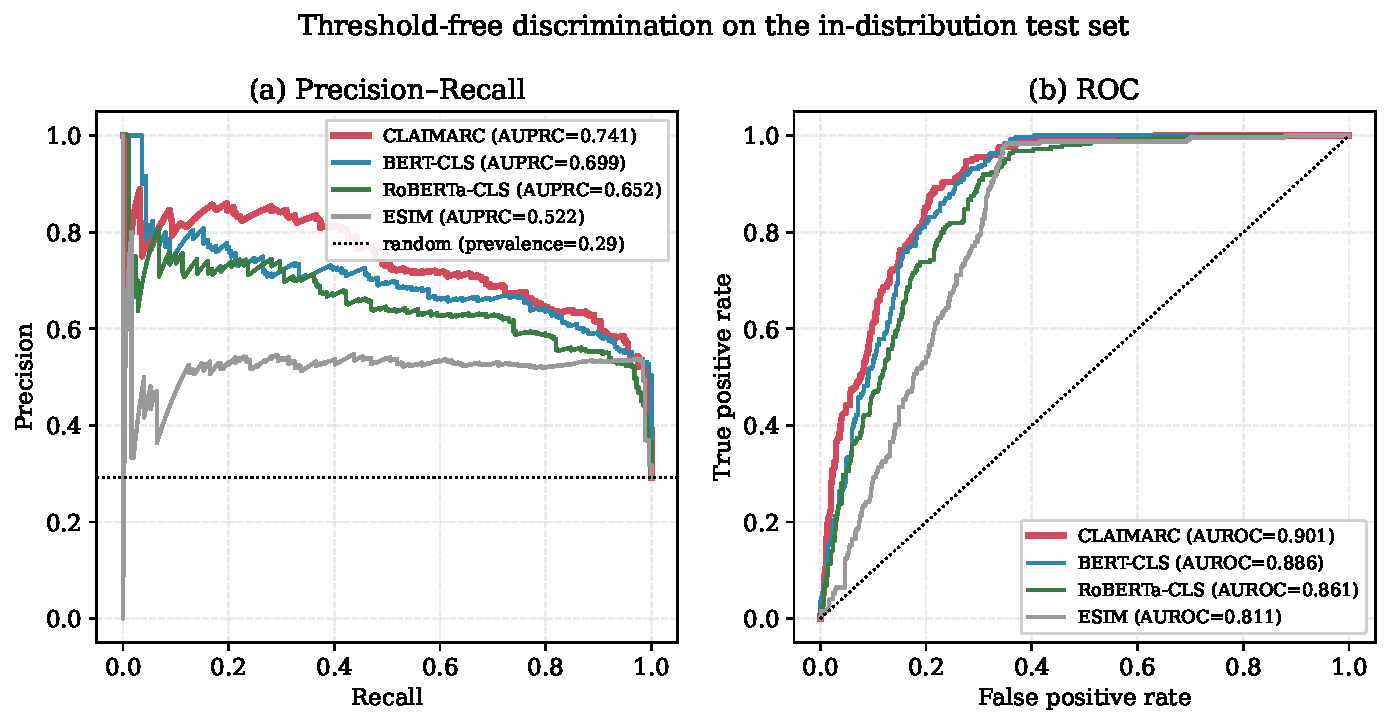
\includegraphics[width=0.86\textwidth]{figs/fig_pr_roc.pdf}
\caption{Threshold-free discrimination on the test set. CLAIMARC (red)
leads the precision--recall curve, most visibly in the high-recall screening
region, and the ROC curve. The dotted line in (a) marks the positive
prevalence (0.29).}
\label{fig:prroc}
\end{figure*}

\subsection{Cross-Domain Generalization (RQ3)}
\label{sec:exp:xdom}

We turn the deployment claim into a test. Every system is trained on the source
domains and evaluated on an unseen target with no target adaptation; CLAIMARC's
retrieval library is built only from the source pairs.
Table~\ref{tab:xdom} reports Accuracy, AUC, AP, and positive-class F1 under
two protocols. The comparison spans all four paradigms, including the two
language-model prompting modes.

Under \textbf{leave-one-category} transfer, where each of the 10 first-level
categories is held out in turn and the result is averaged over the 10 folds,
CLAIMARC is best on Accuracy (81.8), AUC (90.0), and AP (71.0), and holds the
smallest spread across categories (AUC standard deviation 4.0 against
BERT-CLS's 4.7). The best fine-tuned competitor, BERT-CLS, reads 89.4 AUC and
70.1 AP; CLAIMARC keeps a one-point ranking edge while transferring through a
source-only library, so the advantage comes from the structural prior rather
than from re-fitting parameters to the target. Under
\textbf{leave-20-streamers} transfer, where a fixed set of 20
comment-volume-stratified rooms is held out and the result is averaged over
three seeds, CLAIMARC leads both ranking metrics by a clear margin---AUC 93.1
and AP 81.4, against BERT-CLS (92.2/78.7) and RoBERTa-CLS (92.0/78.9)---and stays
within seed noise of the best encoder on the threshold-point metrics (Accuracy
84.2 versus RoBERTa-CLS's 84.5; F1 73.4). The AP lead of roughly 2.5 points over
the strongest encoder is wider than in distribution, which says the attribute
structure CLAIMARC encodes carries across streamers even when speaking style does
not. Under both protocols the zero-shot and five-shot language models stay near
or below random (AUC $\le 0.52$), so a general model's parametric prior does not
transfer to the consumer-perception axis. The consistent thread is that
CLAIMARC's edge is concentrated in ranking quality (AP, AUC) and survives both
forms of distribution shift, which is exactly the regime a screening tool
faces.

\begin{table}[t]
\centering\small
\setlength{\tabcolsep}{6pt}
\newcommand{\pmsd}[1]{\,{\scriptsize$\pm$#1}}
\begin{tabular}{lcccc}
\toprule
\textbf{System} & \textbf{Acc} & \textbf{AUC} & \textbf{AP} & \textbf{F1} \\
\midrule
\multicolumn{5}{l}{\textit{(a) Leave-one-category (mean$\pm$s.d.\ over 10 folds)}} \\
ESIM           & 79.3\pmsd{7.2} & 85.1\pmsd{6.7} & 56.5\pmsd{12.2} & \best{70.1}\pmsd{8.6} \\
BERT-CLS       & 81.0\pmsd{6.5} & 89.4\pmsd{4.7} & 70.1\pmsd{8.0} & 67.5\pmsd{5.0} \\
RoBERTa-CLS    & 81.0\pmsd{4.6} & 88.5\pmsd{4.3} & 67.3\pmsd{6.7} & 66.2\pmsd{8.1} \\
LLM zero-shot  & 49.6\pmsd{3.8} & 45.2\pmsd{5.1} & 25.6\pmsd{12.6} & 29.0\pmsd{13.1} \\
LLM 5-shot CoT & 46.0\pmsd{4.8} & 45.6\pmsd{4.5} & 25.7\pmsd{12.1} & 30.6\pmsd{12.6} \\
\textbf{CLAIMARC} & \best{81.8}\pmsd{5.0} & \best{90.0}\pmsd{4.0} & \best{71.0}\pmsd{5.5} & 66.8\pmsd{5.2} \\
\midrule
\multicolumn{5}{l}{\textit{(b) Leave-20-streamers (mean$\pm$s.d.\ over 3 seeds)}} \\
ESIM           & 82.9\pmsd{1.0} & 88.2\pmsd{0.4} & 68.4\pmsd{0.7} & \best{77.0}\pmsd{1.9} \\
BERT-CLS       & 83.6\pmsd{1.3} & 92.2\pmsd{0.0} & 78.7\pmsd{0.3} & 73.3\pmsd{5.2} \\
RoBERTa-CLS    & \best{84.5}\pmsd{0.4} & 92.0\pmsd{0.2} & 78.9\pmsd{0.8} & 75.6\pmsd{1.4} \\
LLM zero-shot  & 49.0 & 47.0 & 29.3 & 31.7 \\
LLM 5-shot CoT & 48.8 & 52.1 & 32.4 & 43.3 \\
\textbf{CLAIMARC} & 84.2\pmsd{1.3} & \best{93.1}\pmsd{0.3} & \best{81.4}\pmsd{1.3} & 73.4\pmsd{3.7} \\
\bottomrule
\end{tabular}
\caption{Cross-domain generalization (\%) under two protocols, reporting
Accuracy, AUC, AP, and positive-class F1. All systems train on the source and
test on an unseen target with no target adaptation; CLAIMARC's retrieval library
is built only from the source pairs. Panel (a) reports the mean $\pm$ standard
deviation across the 10 held-out first-level categories; panel (b) reports the
mean $\pm$ standard deviation across three seeds for a fixed set of 20
held-out, comment-volume-stratified rooms. The learned systems are compared with
the two language-model prompting modes (run once). CLAIMARC leads on the ranking
metrics (AP, AUC) under both protocols and holds the tightest category spread
(AUC $90.0\pm4.0$ versus BERT-CLS $89.4\pm4.7$); under streamer transfer it is
within seed noise of the best encoder on Accuracy and F1 while leading AP by
$\sim$2.5 points. The in-domain reference AP is 75.4
(Section~\ref{sec:exp:main}). Best per column among the learned systems within
each panel in bold.}
\label{tab:xdom}
\end{table}

The comparison above freezes every system and reads it once on the target. The
framework, however, claims something stronger: that a \emph{frozen} CLAIMARC can
keep improving on a new domain by maintenance of its retrieval index alone, with
no gradient step. We test this directly under streamer transfer. The encoder is
trained on the source rooms and then frozen; we then write a growing fraction of
the held-out streamers' labelled pairs into the retrieval library and re-read the
retrieval vote on the remaining held-out streamers, which are
never written. The forward classifier is fixed throughout---being parametric, it
cannot absorb the new rooms without re-training---so it serves as the
no-adaptation reference. Table~\ref{tab:inject} traces the result. The retrieval
vote, the one component that can adapt, climbs monotonically as the index fills:
AP rises from 65.5 with a source-only library to 71.5 at full target coverage
($+6.0$), AUC from 80.3 to 84.8 ($+4.5$), and the operating-point F1 from 72.4 to
74.9, overtaking the frozen forward classifier's F1 (73.5) once the library is
filled. Crucially the gain is smooth and shows up early---half of it is realized
once only a fifth of the target pool is in the index---so a deployment can absorb
a new streamer or a new risk phrasing incrementally, at the cost of one encode
and a write per pair. This is the concrete mechanism behind the deployment
argument: because RACL has shaped the embedding space so that perceived-risk
structure is locally consistent, dropping a handful of target exemplars into the
neighborhood is enough to re-point the vote, whereas a parametric model would
need a fresh training pass to move at all.

\begin{table}[t]
\centering\small
\setlength{\tabcolsep}{8pt}
\newcommand{\pmsd}[1]{\,{\scriptsize$\pm$#1}}
\begin{tabular}{lccc}
\toprule
\textbf{Retrieval library on held-out streamers} & \textbf{AP} & \textbf{AUC} & \textbf{F1} \\
\midrule
Frozen forward classifier (no adaptation) & 81.1\pmsd{0.9} & 93.1\pmsd{0.3} & 73.5\pmsd{2.9} \\
\midrule
\quad source pairs only                    & 65.5\pmsd{1.8} & 80.3\pmsd{2.6} & 72.4\pmsd{1.9} \\
\quad $+\,20\%$ of target pool             & 67.5\pmsd{1.1} & 81.3\pmsd{2.2} & 73.3\pmsd{1.9} \\
\quad $+\,40\%$                            & 69.0\pmsd{1.2} & 82.7\pmsd{1.7} & 73.8\pmsd{2.6} \\
\quad $+\,60\%$                            & 69.7\pmsd{1.0} & 83.3\pmsd{1.8} & 73.6\pmsd{2.4} \\
\quad $+\,80\%$                            & 70.7\pmsd{1.2} & 84.3\pmsd{1.6} & 74.4\pmsd{2.6} \\
\quad $+\,100\%$ of target pool            & \best{71.5}\pmsd{1.5} & \best{84.8}\pmsd{1.5} & \best{74.9}\pmsd{2.5} \\
\bottomrule
\end{tabular}
\caption{Gradient-free library adaptation under leave-20-streamers transfer
(\%, mean $\pm$ s.d.\ over 3 seeds). The encoder is frozen after source training;
a growing fraction of the held-out streamers' labelled pairs is written into the
retrieval library, and the retrieval vote is read on the
disjoint, never-written half of the held-out streamers. The vote---the only
adaptable component---improves monotonically with library coverage and overtakes
the frozen forward classifier on F1 at full coverage, without any gradient step.}
\label{tab:inject}
\end{table}

\begin{figure}[t]
\centering
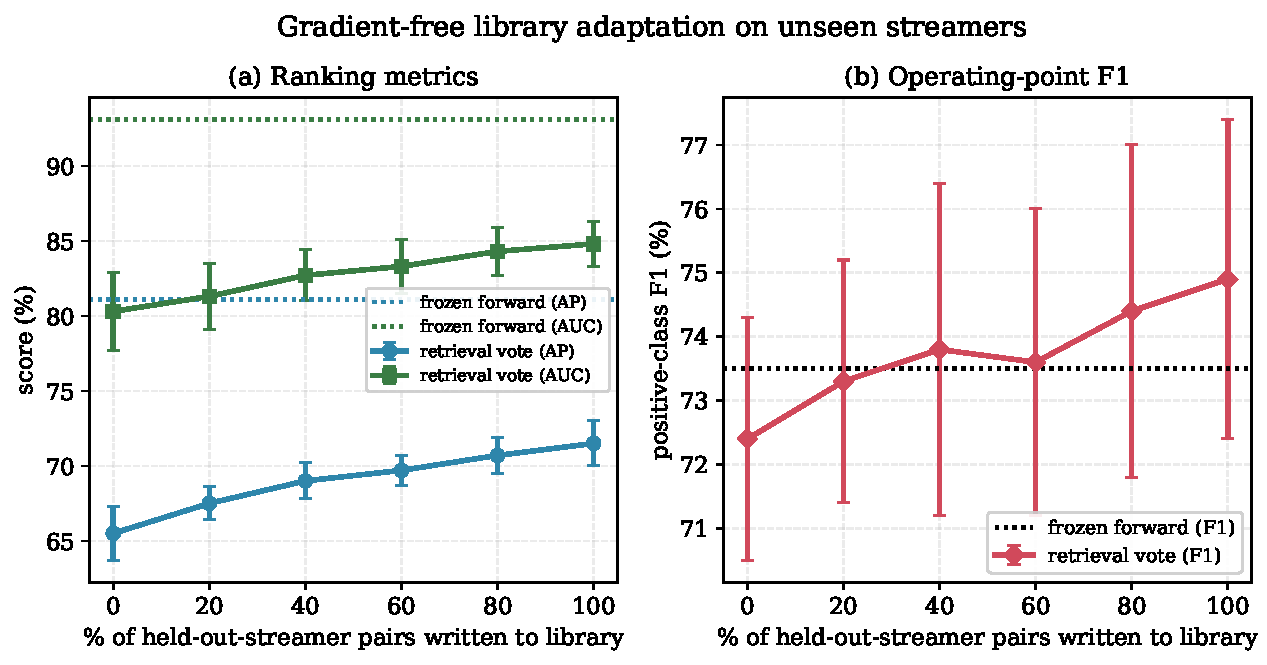
\includegraphics[width=0.86\columnwidth]{figs/fig_inject.pdf}
\caption{Gradient-free library adaptation (leave-20-streamers, 3-seed
mean$\pm$s.d.). As held-out-streamer pairs are written into the frozen-encoder
retrieval library, the retrieval vote's AP and AUC climb monotonically toward the
frozen forward classifier, demonstrating that new streamers are absorbed by index
maintenance rather than re-training.}
\label{fig:xdom}
\end{figure}

\subsection{Representation Geometry and Boundary Sensitivity (RQ2)}
\label{sec:exp:geom}

The value of a contrastive objective should show up in how it reshapes the label
geometry, making misleading and honest pairs more separable in the retrieval
space---the structure the RKC vote (Section~\ref{sec:exp:xdom}) and the
gradient-free library write read off. To separate this effect from prior work we
run a strictly controlled comparison: an identical BGE-full-fine-tuning backbone,
classifier head and hyper-parameters, with three variants that differ \emph{only}
in the contrastive objective---\emph{no contrast} (BCE only), standard supervised
contrastive learning (\emph{SupCon}; Khosla et al.\ 2020, with in-batch
same-label positives and other-label negatives, no retrieval or hard mining), and
our retrieval-augmented contrast (\emph{RACL}; full-pool pseudo-gold positives and
hard negatives, reliability- and class-weighted). All metrics are measured on the
test embeddings $\mathbf{g}_{p,a}$ over three seeds and are attribute-free (the
train split serves as the retrieval index, the test split as queries);
Table~\ref{tab:geom} reports them.

Three findings emerge. First, \textbf{class separability}: RACL reaches a label
silhouette of 0.422, above standard SupCon (0.349) and no-contrast (0.196), and
with the smallest variance ($\pm$0.010 vs.\ SupCon's $\pm$0.173)---the most stable
separation of the three. The UMAP projection in Figure~\ref{fig:umap} shows this
by eye: RACL condenses the misleading pairs into a detached cluster, the two
classes interleave without contrast, and standard SupCon sits in between. Second,
the \textbf{key difference between RACL and standard SupCon is whether the
representation collapses}: SupCon attains the tightest same-label alignment
(0.478) but at the cost of uniformity (only $-0.86$), squeezing same-class points
together; RACL instead keeps the space spread out (uniformity $-1.21$) while
separating the classes, landing in the retrieval-friendlier regime of the
alignment--uniformity plane and avoiding the collapse of the vanilla objective
(Wang and Isola 2020). Third, the \textbf{hard region}: restricted to the
confusable subset (queries whose nearest opposite-label neighbor is most similar),
both contrastive objectives lift neighborhood purity from 0.50 to 0.57---the
contrastive signal acts precisely on pairs that look alike yet carry opposite
labels, which is where RACL applies explicit pressure through hard negatives. We
note that neighborhood purity@10 is comparable across the three ($\approx$0.81):
full fine-tuning already establishes label-consistent neighborhoods, so the
distinct contribution of the contrastive objective is class \emph{separation},
not raw neighbor purity. Taken together, contrastive training yields a more
separable yet uncollapsed retrieval geometry---the structure that the retrieval
vote and library-write adaptation depend on, and the reason the frozen-encoder
vote becomes useful only after the representation is reshaped
(Section~\ref{sec:exp:xdom}).

\begin{table}[t]
\centering\small
\setlength{\tabcolsep}{5pt}
\begin{tabular}{lccccc}
\toprule
\textbf{Variant} & \textbf{Silh.} $\uparrow$ & \textbf{Hard pur.@10} $\uparrow$ & \textbf{Align.} $\downarrow$ & \textbf{Unif.} & \textbf{Pur.@10} \\
\midrule
w/o contrast              & 0.196\std{0.053} & 0.500\std{0.043} & 1.121 & $-2.02$ & 0.811 \\
SupCon (Khosla et al.\ 2020) & 0.349\std{0.173} & \best{0.573\std{0.017}} & 0.478 & $-0.86$ & 0.804 \\
\textbf{RACL (ours)}      & \best{0.422\std{0.010}} & \best{0.573\std{0.088}} & 0.905 & $-1.21$ & 0.811 \\
\bottomrule
\end{tabular}
\caption{Label-conditional geometry of the test retrieval embedding under three
contrastive objectives that share an identical BGE-full-fine-tuning backbone,
classifier and hyper-parameters (3-seed mean$\pm$s.d.; attribute-free, with the
train split as the retrieval index). RACL attains the best and most stable label
silhouette; standard SupCon reaches the tightest alignment but a collapsed (least
uniform) space, whereas RACL preserves uniformity while separating the classes.
Neighborhood purity@10 is already established by full fine-tuning and is
comparable across objectives.}
\label{tab:geom}
\end{table}

\begin{figure}[t]
\centering
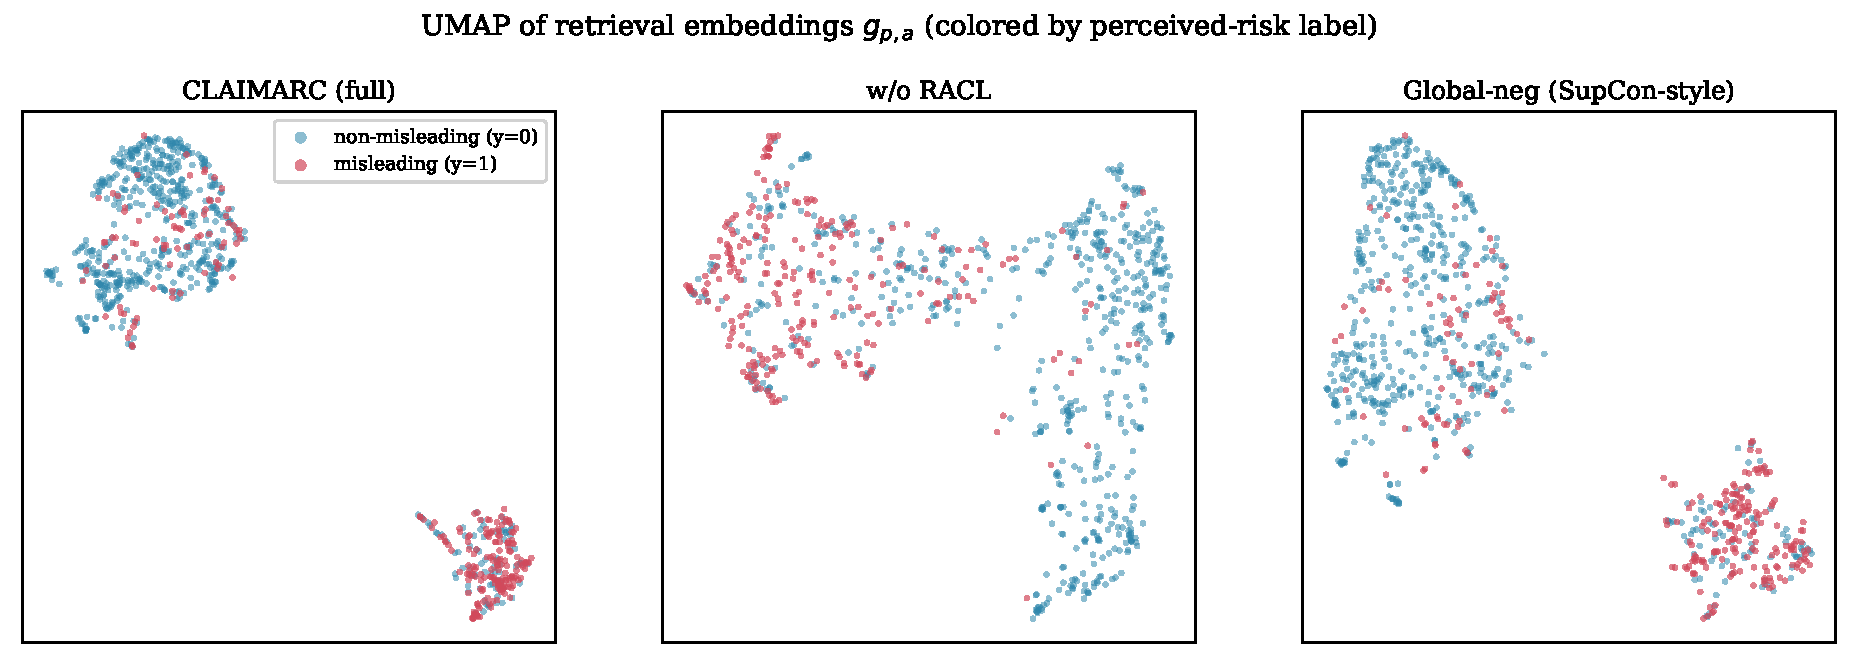
\includegraphics[width=\columnwidth]{figs/fig_umap_label.pdf}
\caption{UMAP of the test retrieval embedding $\mathbf{g}_{p,a}$, colored by
perceived-risk label, under the three contrastive objectives (w/o contrast \textbar{}
SupCon 2020 \textbar{} RACL). RACL isolates the misleading pairs into a detached
cluster; without contrast the two classes interleave, while standard SupCon lies
in between.}
\label{fig:umap}
\end{figure}

\subsection{Ablation Studies (RQ4)}
\label{sec:exp:abl}

We dissect the framework one design choice at a time on the fully fine-tuned
canonical, holding everything else fixed and scoring the forward classifier so
that all variants sit on the same footing. We
follow the organization of recent retrieval-contrastive work (Mei et al.\ 2024)
and report three focused tables, each isolating one family of choices: the core
objective, weighting, and backbone components (Table~\ref{tab:abl}), the
dual-stream architecture (Table~\ref{tab:abl_stream}), and the
retrieval-augmented contrast's positive/negative mining
(Table~\ref{tab:abl_racl}). All numbers are mean $\pm$ standard
deviation over three seeds; the canonical is the bold reference in each table.

\paragraph{Core objective, weighting, and backbone components.}
Table~\ref{tab:abl} removes one component at a time, and every change costs both
the operating point and the ranking metric. Dropping the retrieval-augmented
contrast (cross-entropy only) costs 2.6 F1 (73.4$\to$70.8) and 3.3 AP; removing the
reliability weight that down-weights noisy labels costs 1.8 F1 and 3.2 AP; and
turning off the class-balanced scaling of the contrast---the imbalance-aware
refinement that keeps the 26\% misleading class from being swamped---costs 0.7 F1
and 1.5 AP. Collapsing the classifier and retrieval head's ESIM-style four-tuple
$[\mathbf{h}_c,\mathbf{h}_e,\mathbf{h}_c-\mathbf{h}_e,\mathbf{h}_c\odot\mathbf{h}_e]$
to a plain concatenation $[\mathbf{h}_c,\mathbf{h}_e]$ costs 3.6 AP and 1.4 F1, so
the explicit difference and product features---the discrepancy signal between a
claim and its evidence---are not redundant with what the fusion carries. Swapping
the retrieval-pretrained BGE for BERT-base costs 4.3 AP, confirming that the
ranking draws on the backbone's retrieval pre-training rather than raw encoder
size. The contrast's full value is clearest where a head cannot compensate: the
non-parametric probe in Table~\ref{tab:main}---a reliability-weighted vote on
\emph{frozen} BGE pair embeddings---reaches only 64.4 AP, against 75.4 for the
contrastively trained encoder, and the cross-domain library study in
Section~\ref{sec:exp:xdom} shows the same vote becoming useful only after the
contrast has shaped the space.

\paragraph{Why two contrasting streams.}
Table~\ref{tab:abl_stream} probes the architecture that gives the framework its
name. We compare the canonical dual-stream model against three reductions: keeping
both streams but removing the cross-attention TwoStreamFusion (concatenation
only), and two genuine single-stream models that feed only the claim or only the
evidence into the encoder with no fusion at all. The evidence-only model
\emph{collapses}---AP falls to 48.4 and AUC to 68.7, barely above the 29.1\%
prevalence---because the perceived-risk label lives in whether the evidence
\emph{contradicts the claim}, a relation that is unreadable once the claim is
removed. The claim-only model fares better but still loses 5.0 AP, since without
the evidence it cannot tell an honest claim from an unsupported one. With both
streams present, removing the fusion still costs 4.6 F1 and 1.9 Accuracy---the
largest operating-point drop among all variants---confirming that the cross-stream
interaction, not merely the presence of two encoders, is what aligns a claim with
its evidence. The two streams and their interaction are jointly necessary.

\paragraph{Retrieval-augmented contrast: which examples to draw.}
Table~\ref{tab:abl_racl} ablates the positive and negative mining of the contrast,
following the protocol of RGCL (Mei et al.\ 2024). Two choices that the literature
warns about are confirmed here. First, replacing the pseudo-gold positives
(highest-similarity same-label neighbors) with hard positives (lowest-similarity
same-label neighbors) does not help and slightly lowers F1 (73.0 vs 73.4),
matching the report that hard positives destabilize retrieval-guided contrast.
Second, restricting negatives---either to same-attribute pairs or to the same
evidence type---never beats the simpler class-balanced global pool, so the
canonical keeps the global pool. The number of pseudo-gold positives is inert
(Kp $\in\{1,3,5\}$ all within noise), but the number of hard negatives has a clear
optimum: too few (Kn$=1$) costs 1.3 F1 and too many (Kn$=10$) costs 4.2 F1, so the
canonical Kn$=5$ is the sweet spot, echoing the finding that piling on hard
negatives degrades retrieval-contrastive training.

\begin{table}[t]
\centering\small
\setlength{\tabcolsep}{6pt}
\newcommand{\pmsd}[1]{\,{\scriptsize$\pm$#1}}
\begin{tabular}{lcccc}
\toprule
\textbf{Variant (CLAIMARC, forward)} & \textbf{Acc} & \textbf{F1} & \textbf{AP} & \textbf{AUC} \\
\midrule
\textbf{Canonical CLAIMARC}          & \best{82.6}\pmsd{0.4} & \best{73.4}\pmsd{0.5} & \best{75.4}\pmsd{1.3} & \best{90.4}\pmsd{0.4} \\
\midrule
\quad w/o RACL contrast (CE only)    & 81.2\pmsd{1.1} & 70.8\pmsd{2.0} & 72.1\pmsd{2.3} & 89.4\pmsd{0.9} \\
\quad w/o reliability weight $c$     & 81.6\pmsd{1.3} & 71.6\pmsd{1.6} & 72.2\pmsd{3.1} & 89.5\pmsd{0.7} \\
\quad w/o class-balanced contrast    & 82.1\pmsd{0.5} & 72.7\pmsd{1.9} & 73.9\pmsd{0.4} & 89.9\pmsd{0.2} \\
\quad w/o ESIM 4-tuple head (concat only) & 81.4\pmsd{0.6} & 72.0\pmsd{1.7} & 71.8\pmsd{2.3} & 89.4\pmsd{0.5} \\
\quad backbone: BGE $\to$ BERT       & 81.2\pmsd{0.6} & 72.4\pmsd{0.9} & 71.1\pmsd{1.4} & 89.2\pmsd{0.4} \\
\bottomrule
\end{tabular}
\caption{Core objective, weighting, and backbone components, removed one at a time
(\%, forward classifier, mean $\pm$ s.d.\ over three seeds; canonical in bold).
Every removal lowers both the operating point and the ranking metric, locating
the contribution of each component.}
\label{tab:abl}
\end{table}

\begin{table}[t]
\centering\small
\setlength{\tabcolsep}{6pt}
\newcommand{\pmsd}[1]{\,{\scriptsize$\pm$#1}}
\begin{tabular}{lcccc}
\toprule
\textbf{Stream design} & \textbf{Acc} & \textbf{F1} & \textbf{AP} & \textbf{AUC} \\
\midrule
\textbf{Dual-stream + TwoStreamFusion} & \best{82.6}\pmsd{0.4} & \best{73.4}\pmsd{0.5} & \best{75.4}\pmsd{1.3} & \best{90.4}\pmsd{0.4} \\
\midrule
\quad Dual-stream, w/o fusion (concat) & 80.7\pmsd{0.5} & 68.8\pmsd{3.2} & 73.8\pmsd{1.4} & 89.6\pmsd{0.4} \\
\quad Claim stream only (no fusion)    & 81.1\pmsd{1.0} & 73.0\pmsd{0.3} & 70.4\pmsd{1.9} & 89.2\pmsd{0.1} \\
\quad Evidence stream only (no fusion) & 68.7\pmsd{0.8} & 44.1\pmsd{4.3} & 48.4\pmsd{0.4} & 68.7\pmsd{1.2} \\
\bottomrule
\end{tabular}
\caption{Necessity of two contrasting streams (\%, forward classifier, mean
$\pm$ s.d.\ over three seeds; canonical in bold). A single stream cannot read the
claim--evidence relation: the evidence-only model collapses to near-prevalence AP,
and even with both streams the cross-attention fusion is needed for the operating
point.}
\label{tab:abl_stream}
\end{table}

\begin{table}[t]
\centering\small
\setlength{\tabcolsep}{6pt}
\newcommand{\pmsd}[1]{\,{\scriptsize$\pm$#1}}
\begin{tabular}{lcccc}
\toprule
\textbf{RACL retrieval design} & \textbf{Acc} & \textbf{F1} & \textbf{AP} & \textbf{AUC} \\
\midrule
\textbf{Pseudo-gold pos., global hard neg. (Kp3/Kn5)} & \best{82.6}\pmsd{0.4} & \best{73.4}\pmsd{0.5} & \best{75.4}\pmsd{1.3} & \best{90.4}\pmsd{0.4} \\
\midrule
\multicolumn{5}{l}{\emph{Positive / negative type}}\\
\quad hard positives (vs pseudo-gold)      & 81.9\pmsd{1.1} & 73.0\pmsd{0.7} & 73.7\pmsd{0.7} & 90.0\pmsd{0.2} \\
\quad same-attribute negatives             & 82.1\pmsd{0.4} & 72.6\pmsd{1.3} & 73.5\pmsd{0.5} & 90.0\pmsd{0.0} \\
\quad same-evidence-type negatives         & 81.8\pmsd{0.3} & 72.7\pmsd{1.5} & 74.0\pmsd{0.5} & 90.0\pmsd{0.1} \\
\midrule
\multicolumn{5}{l}{\emph{Number of retrieved examples}}\\
\quad positives Kp$=1$                     & 82.5\pmsd{0.7} & 73.4\pmsd{0.6} & 74.0\pmsd{0.7} & 89.9\pmsd{0.2} \\
\quad positives Kp$=5$                     & 82.4\pmsd{0.5} & 73.4\pmsd{0.2} & 73.7\pmsd{0.5} & 90.0\pmsd{0.1} \\
\quad hard negatives Kn$=1$                & 81.4\pmsd{0.4} & 72.1\pmsd{1.4} & 73.6\pmsd{0.2} & 90.0\pmsd{0.1} \\
\quad hard negatives Kn$=10$               & 81.1\pmsd{0.3} & 69.2\pmsd{2.3} & 73.5\pmsd{0.4} & 89.9\pmsd{0.1} \\
\bottomrule
\end{tabular}
\caption{Retrieval-augmented contrast: positive/negative mining, in the protocol
of RGCL (Mei et al.\ 2024) (\%, forward classifier, mean $\pm$ s.d.\ over three seeds;
canonical in bold). Pseudo-gold positives beat hard positives, restricting
negatives never helps, and the hard-negative count has a clear optimum at five.}
\label{tab:abl_racl}
\end{table}

\subsection{Does the Reliability Weight Earn Its Form? (RQ4)}
\label{sec:exp:cval}

The reliability weight $c_{p,a}$ is one of the components that moves the headline
in Table~\ref{tab:abl}, so we ask a sharper question than ``does it help'': is its
\emph{specific} construction warranted, or would any down-weighting of low-signal
pairs do? We answer with a controlled study that holds the architecture and the
data fixed and perturbs only the per-sample training weight $w_{p,a}$, leaving
the validation- and test-set weights untouched so the threshold and the
weighted metrics stay comparable across rows. Table~\ref{tab:cval} reports the
forward classifier under seven counterfactual weightings. The reading is
consistent. Removing the weight (uniform) costs 2.2 F1, in line with the
ablation. \emph{Reversing} it---up-weighting the pairs the design judges
least reliable---costs 5.7 F1 and lands below uniform, so the direction of the
weight, not merely its presence, carries information: a high $c$ does mark a
more trustworthy label. Randomly \emph{permuting} $c$ across pairs, which keeps
its marginal distribution but destroys the pair-to-weight correspondence, falls
back to the uniform level, so the value is in \emph{which} pairs are
up-weighted, not in the shape of the weight histogram. Coarsening $c$ to a
median split (binary) is the counterfactual that moves the ranking metrics most,
dropping AP by 7.0, which says the continuous grading---not just a
reliable/unreliable dichotomy---is what protects the precision--recall ordering.
Collapsing the composite to its saturation term alone (count) costs 1.5 F1, so
the asymmetric-diagnosticity and authenticity factors contribute beyond a raw
comment count, and rolling back to the pre-refinement label weights (old $c$)
costs 3.4 F1, so the label-reconstruction iteration was not cosmetic. The lone
neutral perturbation is a square-root reshaping, which preserves the ordering
and matches the canonical within noise---the design is robust to how steeply it
grades reliability but highly sensitive to reversing, flattening, or
shuffling it. Two patterns cut across the table: the operating-point metrics
(Accuracy, F1) consistently favor the canonical weight while the threshold-free
metrics barely move except under binarization, which locates the mechanism
precisely---reliability weighting sharpens the decision boundary rather than
re-ranking the test set.

\begin{table}[t]
\centering\small
\setlength{\tabcolsep}{7pt}
\newcommand{\pmsd}[1]{\,{\scriptsize$\pm$#1}}
\begin{tabular}{lcccc}
\toprule
\textbf{Training weight $w_{p,a}$} & \textbf{Acc} & \textbf{F1} & \textbf{AP} & \textbf{AUC} \\
\midrule
\textbf{Canonical} ($w{=}c$, the design) & \best{82.6}\pmsd{0.4} & 73.4\pmsd{0.5} & \best{75.4}\pmsd{1.3} & \best{90.4}\pmsd{0.4} \\
\midrule
Uniform ($w{=}1$)               & 81.6\pmsd{1.2} & 71.2\pmsd{1.6} & 73.3\pmsd{2.3} & 89.6\pmsd{0.6} \\
Reversed                        & 80.0\pmsd{0.4} & 67.7\pmsd{3.5} & 74.1\pmsd{1.9} & 89.5\pmsd{0.3} \\
Permuted across pairs           & 80.4\pmsd{0.6} & 71.6\pmsd{1.5} & 73.0\pmsd{2.8} & 89.4\pmsd{0.8} \\
Median-split (binary)           & 79.5\pmsd{0.8} & 70.2\pmsd{2.5} & 68.4\pmsd{1.1} & 88.3\pmsd{0.7} \\
Saturation term only            & 80.3\pmsd{0.3} & 71.9\pmsd{0.4} & 73.1\pmsd{1.6} & 89.1\pmsd{0.4} \\
Pre-refinement (old $c$)        & 80.4\pmsd{1.3} & 70.0\pmsd{3.4} & 72.1\pmsd{0.8} & 89.4\pmsd{0.6} \\
Square-root ($w{=}\sqrt{c}$)    & 81.8\pmsd{1.5} & \best{74.0}\pmsd{1.3} & 72.6\pmsd{2.5} & 89.9\pmsd{0.5} \\
\bottomrule
\end{tabular}
\caption{Counterfactual reliability weightings (\%, forward classifier, mean
$\pm$ s.d.\ over three seeds). Only the per-sample \emph{training} weight is
altered; validation/test weights and the architecture are held fixed. The
canonical weight $w{=}c$ is best on Accuracy, AP, and AUC, with the square-root
reshaping tying it on F1; the threshold-free metrics are insensitive to loss
re-weighting except under the coarse median split, which breaks the
precision--recall ordering (AP $-7.0$). Reversing the weight is worse than
removing it, and permuting it reverts to the uniform level---the design's value
is sample-specific and directional, not a generic down-weighting.}
\label{tab:cval}
\end{table}

\subsection{Hyper-parameter Sensitivity and Efficiency (RQ4)}
\label{sec:exp:hyper}

Figure~\ref{fig:hparam} sweeps five core knobs: the number of fusion blocks
$N$, the number of attention heads, the LoRA rank, the contrastive temperature
$\tau$, and the retrieval sizes $(K_p,K_n)$; Table~\ref{tab:sweep} in the
appendix lists these together with the loss-function, feed-forward,
cross-attention, and projection variants, for 26 single-seed configurations in
all; to keep the sweep affordable these runs use the parameter-efficient
LoRA-frozen variant. AP stays inside a narrow 0.69--0.74 band across the five
core knobs. The canonical objective and retrieval settings
($\lambda_{\mathrm{CL}}{=}0.5$, $\tau{=}0.07$, $N{=}2$, $(K_p,K_n){=}(3,5)$) sit
on the flat part of each curve, and only an oversized retrieval set $(5,10)$
degrades the score by pulling in noisy neighbors. The model is not sensitive to
these choices within a reasonable range, which is why the configuration was
fixed once on the validation set rather than tuned per metric.

Table~\ref{tab:eff} compares deployment costs. The canonical CLAIMARC fully
fine-tunes its 396.5M parameters and finishes the two-stage schedule in about
18 minutes on one RTX~4090; at inference it encodes a pair in 36\,ms and runs
RKC retrieval over the 3{,}636-item library in 0.18\,ms per
query. The parameter-efficient variant trains only 92.7M parameters (23.4\%)
with the backbone frozen, trading about five AP points (Table~\ref{tab:abl}) for
a decisive operational property recorded in the last column: adapting to a new
streamer, category, or risk phrasing costs one 36\,ms encode and a write to the
library, with no gradient step, whereas every parametric baseline---and the
fully fine-tuned canonical itself---needs a retraining pass, and the 7B model
also carries about $20\times$ the parameters and an autoregressive decoding cost.
Moving the adaptable component out of the model weights and into an external
index is what buys this.

\begin{table}[t]
\centering\small
\setlength{\tabcolsep}{6pt}
\begin{tabular}{lrrl}
\toprule
\textbf{System} & \textbf{Total} & \textbf{Trainable} & \textbf{New-domain adaptation} \\
\midrule
BERT-base (FT)         & 102M     & 102M (100\%)          & gradient retrain \\
Qwen2.5-7B+LoRA        & 7{,}616M & ${\sim}20$M           & LoRA retrain \\
CLAIMARC (full)        & 396.5M   & 396.5M (100\%)        & gradient retrain \\
\textbf{CLAIMARC (LoRA-frozen)} & 396.5M & \best{92.7}M (23.4\%) & \textbf{library write} \\
\bottomrule
\end{tabular}
\caption{Deployment cost. The canonical fully fine-tunes the encoder; the
parameter-efficient variant trains a minority of its parameters and absorbs new
domains by a library write (one 36\,ms encode, no gradient step) rather than by
retraining, for about a five-point AP trade-off (Section~\ref{sec:exp:abl}).}
\label{tab:eff}
\end{table}

\begin{figure}[t]
\centering
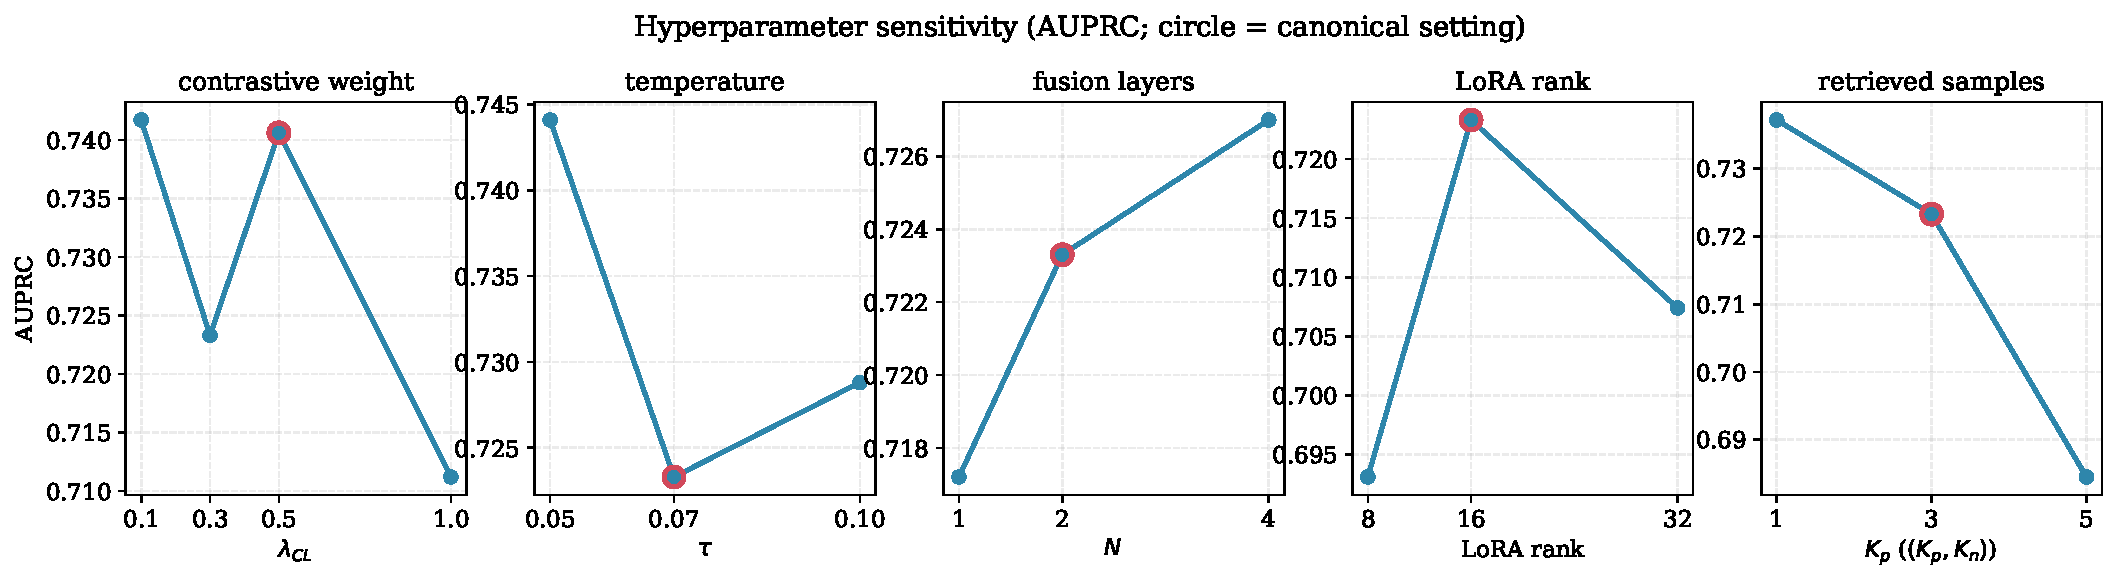
\includegraphics[width=\columnwidth]{figs/fig_hparam.pdf}
\caption{Hyper-parameter sensitivity (AP). Across all five sweeps the score
stays inside a narrow band; the canonical configuration (circled) sits on the
stable plateau.}
\label{fig:hparam}
\end{figure}

\subsection{Selective Prediction and Error Analysis}
\label{sec:exp:select}

A screening tool runs alongside human reviewers, so its value depends not only
on average accuracy but on whether it can flag its own unreliable calls for
escalation. CLAIMARC offers a training-free gate for this. The forward
classifier and the RKC retrieval vote are two near-independent views of the
same pair, and their disagreement $|p_{\mathrm{fwd}}-p_{\mathrm{RKC}}|$ (the
self-consistency signal of \S3.2.9) marks the cases to abstain on and route to
a reviewer. Figure~\ref{fig:selective} traces the risk--coverage trade-off as
we abstain on the most-disagreeing pairs, averaging over the three canonical
seeds. The auto-decided subset improves monotonically: lowering coverage from
100\% to 80\%, by escalating the 20\% of pairs with the largest disagreement,
raises Accuracy from 0.814 to 0.867 and selective AP from 0.737 to 0.778; at 70\%
coverage Accuracy reaches 0.889 and AP 0.809, and at 65\% coverage Accuracy 0.908
and AP 0.835. A random abstention of the same size leaves every metric flat
(Accuracy around 0.81, AP around 0.73), so the gate is isolating genuinely hard cases rather than just
shrinking the set. In effect the model becomes a calibrated triage front-end
that clears the confident majority and surfaces a small, high-yield queue for
human review. The reliability diagram in Figure~\ref{fig:calib} adds that a
single temperature scale brings the predicted probabilities close to the
diagonal, which supports their use in a decision-support setting.

Turning to the errors, at the validation-selected operating point CLAIMARC
recovers 84\% of the perceived-misleading pairs (TP$=$210, FN$=$39), trading
some precision (FP$=$120) as a screening tool should. The errors concentrate
where product evidence is thin: the error rate falls from 24.1\% to 16.4\% to
10.3\% as evidence-source coverage goes from one to two to three sources, which
both supports the three-source product-fact channel and points to evidence
acquisition, rather than the discriminator, as the limit in the residual
regime. Two interpretable error types stand out. False negatives are mostly
terse stylized endorsements such as ``\textit{加绒的}'', ``\textit{质感真的很顶}'',
and ``\textit{版型好看}'' that consumers later judged misleading but that carry
no surface contradiction with the product facts; these are the cases the
fact-verification and LLM baselines also miss, and the limit here is signal
sparsity rather than geometry. False positives concentrate on hyperbolic
metaphor over a benign fact, for example ``\textit{喷上去之后就跟镀了膜似的}'' for
a foam-type product, where the model over-attributes risk to vivid figurative
language. Finally, CLAIMARC and BERT make different mistakes, each correcting
about 44 of the other's errors and agreeing on only 114, which points to
complementary inductive biases and makes a retrieval-augmented ensemble a
natural next step.

\begin{figure}[t]
\centering
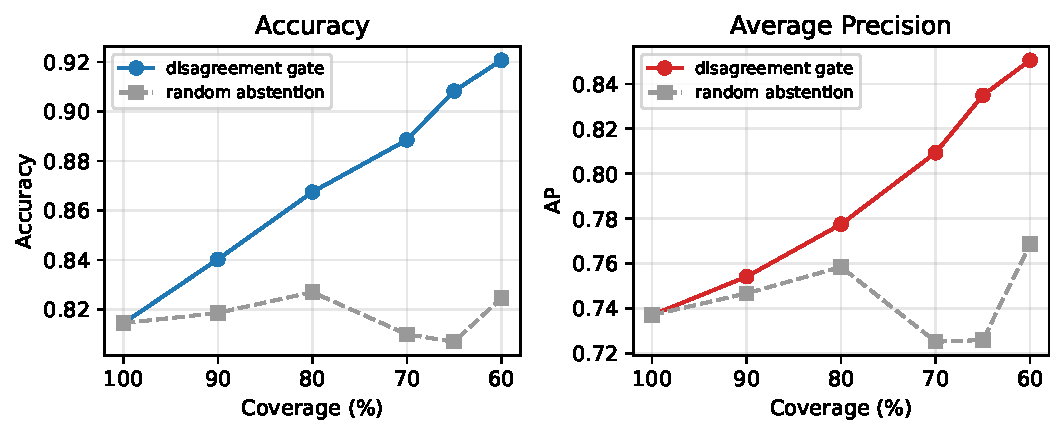
\includegraphics[width=\columnwidth]{figs/fig_selective.pdf}
\caption{Selective prediction on the test set. Abstaining on the highest
forward--RKC disagreement and routing those pairs to human review improves both
selective AP and Accuracy on the auto-decided remainder, whereas a random
abstention of the same size (dashed) stays flat.}
\label{fig:selective}
\end{figure}

\begin{figure}[t]
\centering
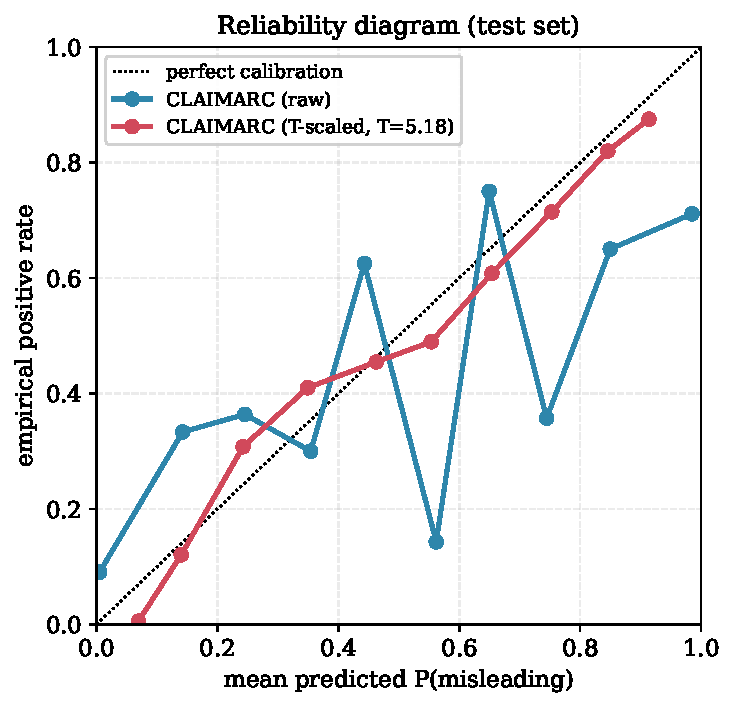
\includegraphics[width=0.82\columnwidth]{figs/fig_calibration.pdf}
\caption{Reliability diagram (test). A single temperature scale brings
CLAIMARC's predicted probabilities close to the diagonal.}
\label{fig:calib}
\end{figure}

\section{Conclusion}
\label{sec:concl}

\subsection{Findings}
\label{sec:concl:find}

The four research questions resolve as follows. On RQ1, CLAIMARC leads on all
four metrics---Accuracy 82.6, F1$_{\text{pos}}$ 73.4, AP 75.4, and AUC
90.4---under the same end-to-end fine-tuning budget as the encoder baselines, with
the widest margins on the threshold-free ranking metrics the framework targets
(AP $+6.4$ over the best fine-tuned encoder). The two competing explanations both fail across
the 14 baselines: objective fact verification is the weakest learned family
(ESIM AP 51.2, a BERT-NLI cross-encoder 67.9), and the zero-shot LLMs sit at or
below random (AP 27--29), with five-shot CoT no better; even a LoRA-fine-tuned
Qwen2.5-7B trails by more than 10 AP at roughly $20\times$ the parameters, and a
non-parametric probe on frozen embeddings reaches only 64.4 AP---it is the
contrastive geometry, not the retrieval rule, that carries the result. On RQ2,
under a controlled comparison against standard supervised contrastive learning
(SupCon; Khosla et al.\ 2020), RACL produces the best and most stable class
separation (label silhouette 0.422 vs.\ 0.349 for SupCon and 0.196 without
contrast) and lifts hard-region neighbor purity from 0.50 to 0.57; unlike standard
SupCon it separates the classes without collapsing the representation (a balanced
alignment--uniformity profile), the geometric structure the retrieval vote and
library write exploit. On RQ3, CLAIMARC transfers best of all learned systems, leading the
ranking metrics on unseen categories (AUC 90.0, AP 71.0) and on unseen streamers
(AUC 93.1, AP 81.4, the largest streamer-transfer AP of any system), while the
LLMs do not transfer at all; freezing the encoder and writing held-out streamer
pairs into the retrieval library then lifts the gradient-free vote monotonically
from 65.5 to 71.5 AP, narrowing the gap to the trained forward classifier without
a single gradient step. On RQ4, three focused ablation tables---core components
and backbone, dual-stream architecture, and retrieval design---each
support the design: removing fusion costs 4.6 F1, removing the contrastive
objective 2.6 F1, and dropping the reliability weighting 1.8 F1; both streams are
necessary (the evidence-only model collapses to 48.4 AP and the claim-only model
loses 5.0 AP); the ESIM four-tuple head and the retrieval-pretrained backbone each
contribute about 3.6 and 4.3 AP; pseudo-gold positives beat hard positives,
restricting negatives never helps, and the hard-negative count is optimal at five;
the non-parametric probe on frozen embeddings collapses to 64.4 AP, while a
parameter-efficient LoRA-frozen variant recovers most of the accuracy at 23\% of
the trainable parameters and enables gradient-free library-write adaptation.
Beyond accuracy, the forward--RKC disagreement gate turns the model into a
calibrated triage front-end, lifting Accuracy from 0.814 to 0.867 at 80\%
coverage while a random abstention does nothing.

\subsection{Contributions}
\label{sec:concl:contrib}

The study contributes on three levels. At the problem level, it redefines
misleading-advertising detection in livestreaming, moving the supervision
anchor from a claim-versus-knowledge-base check to an attribute-level judgment
of consumer-perceived risk grounded in comments, and operationalizes that shift
with a computable binary target and an instance-level reliability weight. The
main comparison and the ablation together show the redefinition is empirically
warranted: the fact-verification family is much weaker, and the fusion,
contrast, and reliability components each carry part of the signal. At the method level, CLAIMARC
folds retrieval-guided contrastive learning into joint claim--evidence
discrimination, indexing the embedding space, drawing neighbors into the
contrastive objective, and concentrating the learning pressure on pairs that
look alike yet carry different labels; against a standard supervised contrastive
baseline, the geometry analysis shows that this yields the best and uncollapsed
class separation, the structure the retrieval vote relies on. At the
deployment level, the framework admits a parameter-efficient variant that freezes
the encoder after training and adapts through library writes, converting the
absorption of new streamers, categories, and risk phrasings from model retraining
into index maintenance at about a five-point AP trade-off; the cross-domain and
efficiency results confirm that this pathway holds, and the disagreement gate
supplies a model$\to$human$\to$data$\to$model loop for compliance review. A few
limits remain. The residual errors are dominated by terse endorsements with no
evidential trace, where the bottleneck is signal acquisition rather than the
model. This points to the next step, namely richer and cleaner evidence channels and
a retrieval-augmented ensemble that combines the complementary errors of CLAIMARC
and a fine-tuned encoder.

\appendix
\section{Hyper-parameter and Variant Sweep}
\label{app:sweep}

Table~\ref{tab:sweep} reports the full single-seed sweep summarized in
Section~\ref{sec:exp:hyper} and Figure~\ref{fig:hparam}. Together with the
three-seed ablation battery in Tables~\ref{tab:abl}--\ref{tab:abl_racl}, it spans capacity (fusion depth, heads, LoRA rank), the
contrastive objective ($\lambda_{\mathrm{CL}}$, $\tau$, retrieval sizes, loss),
architecture (feed-forward activation, cross-attention direction, projection
sharing), and evidence composition. All rows read the forward classifier on the
test set; the canonical configuration is the bold reference.

\begin{table}[h]
\centering\footnotesize
\setlength{\tabcolsep}{6pt}
\begin{tabular}{lcccc}
\toprule
\textbf{Configuration} & \textbf{Acc} & \textbf{F1} & \textbf{AP} & \textbf{AUC} \\
\midrule
\textbf{Canonical} ($N2$, h8, r16, $\lambda.5$, $\tau.07$, $K35$, BCE) & \textbf{80.8} & \textbf{70.5} & \textbf{70.6} & \textbf{88.6} \\
\midrule
\multicolumn{5}{l}{\emph{Fusion blocks} $N$}\\
\quad $N{=}1$ & 80.9 & 72.1 & 72.7 & 89.2 \\
\quad $N{=}3$ & 80.6 & 72.6 & 72.6 & 89.5 \\
\quad $N{=}4$ & 80.2 & 70.8 & 70.0 & 86.9 \\
\multicolumn{5}{l}{\emph{Attention heads}}\\
\quad 4 heads  & 80.5 & 70.0 & 71.0 & 89.0 \\
\quad 16 heads & 79.9 & 70.9 & 70.5 & 88.9 \\
\multicolumn{5}{l}{\emph{LoRA rank}}\\
\quad rank 8  & 80.6 & 71.8 & 70.5 & 89.1 \\
\quad rank 32 & 81.0 & 73.3 & 73.6 & 89.6 \\
\multicolumn{5}{l}{\emph{Contrastive weight} $\lambda_{\mathrm{CL}}$}\\
\quad 0.1 & 79.8 & 70.8 & 69.8 & 88.0 \\
\quad 0.3 & 79.7 & 70.2 & 69.5 & 87.9 \\
\quad 1.0 & 80.6 & 71.4 & 70.3 & 88.3 \\
\multicolumn{5}{l}{\emph{Temperature} $\tau$}\\
\quad 0.05 & 79.9 & 70.5 & 69.6 & 88.0 \\
\quad 0.10 & 79.8 & 70.6 & 69.8 & 88.0 \\
\quad 0.20 & 80.3 & 70.8 & 69.1 & 88.5 \\
\multicolumn{5}{l}{\emph{Retrieval sizes} $(K_p,K_n)$}\\
\quad $(1,1)$  & 79.8 & 70.9 & 70.0 & 88.1 \\
\quad $(5,10)$ & 80.0 & 70.4 & 69.5 & 87.9 \\
\multicolumn{5}{l}{\emph{Loss function}}\\
\quad ASL   & 81.3 & 72.7 & 71.8 & 88.8 \\
\quad Focal & 79.9 & 68.7 & 68.6 & 87.4 \\
\multicolumn{5}{l}{\emph{Architecture}}\\
\quad FFN GeLU (vs.\ SwiGLU)      & 80.0 & 69.7 & 71.7 & 88.7 \\
\quad cross-attn.\ claim$\to$ev.\ & 81.4 & 69.7 & 71.2 & 88.1 \\
\quad cross-attn.\ ev.$\to$claim  & 80.3 & 72.4 & 68.0 & 88.3 \\
\quad independent projections     & 81.3 & 72.8 & 73.6 & 89.8 \\
\multicolumn{5}{l}{\emph{Evidence policy}}\\
\quad source-first               & 79.9 & 70.8 & 69.9 & 88.0 \\
\quad params only                & 82.0 & 72.4 & 74.1 & 89.8 \\
\quad OCR only                   & 80.3 & 68.5 & 75.2 & 89.4 \\
\quad VLM only                   & 81.3 & 73.8 & 75.6 & 90.0 \\
\quad multi-view mix             & 80.0 & 70.6 & 69.9 & 88.1 \\
\bottomrule
\end{tabular}
\caption{Single-seed hyper-parameter and variant sweep (\%, forward classifier,
test set). The five core knobs (fusion depth, heads, LoRA rank, $\tau$,
$(K_p,K_n)$) keep AP in a 0.69--0.74 band; the canonical setting sits on the flat
region. The single-source evidence policies reach high peak AP (up to 75.6) on
individual views, but the canonical mix is kept for coverage and robustness when
a given view is sparse.}
\label{tab:sweep}
\end{table}

\section{Reliability-Weight Formula Sensitivity}
\label{app:cform}

Section~\ref{sec:exp:cval} shows that the reliability weight earns its
\emph{form}; here we close the loop by perturbing the four hyper-parameters
inside the formula itself: the evidence-saturation rate $k$, the asymmetric
diagnosticity discount $\lambda$, the fake-review discount $\rho$, and the
strong-negative bonus $\phi_{\mathrm{bonus}}$. Holding the network and training
fixed, we recompute $c$ with one parameter moved at a time and re-fit a single
seed; Table~\ref{tab:cform} reads the forward classifier. Every excursion from
the chosen $(k{=}3,\lambda{=}0.3,\rho{=}0.4,\phi_{\mathrm{bonus}}{=}1.2)$ lowers
AP relative to the three-seed canonical (75.4), confirming the operating point
was well chosen. The two steepest sensitivities are interpretable: over-saturating
the evidence count ($k{=}6$, AP $67.8$) flattens the distinction between thinly
and richly evidenced pairs, and weakening the strong-negative bonus
($\phi_{\mathrm{bonus}}{=}1.0$, AP $68.8$) removes the up-weighting of pairs with
explicit refuting evidence---both core to what $c$ is meant to encode. The
discount terms $\lambda$ and $\rho$ are flatter, moving AP by at most two points.

\begin{table}[h]
\centering\footnotesize
\setlength{\tabcolsep}{6pt}
\begin{tabular}{llcccc}
\toprule
\textbf{Parameter} & \textbf{Setting} & \textbf{Acc} & \textbf{F1} & \textbf{AP} & \textbf{AUC} \\
\midrule
\multicolumn{2}{l}{\textbf{Canonical} ($k3,\lambda.3,\rho.4,\phi1.2$; 3-seed)} & \textbf{82.6} & \textbf{73.4} & \textbf{75.4} & \textbf{90.4} \\
\midrule
Saturation rate $k$        & 1.5 & 78.7 & 72.4 & 72.6 & 89.3 \\
                           & 6.0 & 79.0 & 63.9 & 67.8 & 88.1 \\
Asym.\ discount $\lambda$  & 0.1 & 81.2 & 73.9 & 71.6 & 89.5 \\
                           & 0.6 & 80.5 & 68.8 & 72.3 & 89.1 \\
Fake-review disc.\ $\rho$  & 0.2 & 81.8 & 70.7 & 72.1 & 89.5 \\
                           & 0.6 & 80.9 & 70.4 & 70.0 & 88.8 \\
Strong-neg bonus $\phi$    & 1.0 & 78.6 & 72.0 & 68.8 & 88.7 \\
                           & 1.5 & 81.6 & 70.8 & 71.2 & 89.2 \\
\bottomrule
\end{tabular}
\caption{Reliability-weight formula sensitivity (\%, forward classifier, test
set). One hyper-parameter of the $c$ construction is moved at a time and $c$ is
recomputed; rows are single seed, the canonical is the three-seed reference.
Every excursion lowers AP, with the saturation rate $k$ and the strong-negative
bonus $\phi_{\mathrm{bonus}}$ the most sensitive.}
\label{tab:cform}
\end{table}

\begin{thebibliography}{99}
\small
\bibitem{chen2017} Chen Q, Zhu X, Ling Z, Wei S, Jiang H, Inkpen D (2017)
Enhanced LSTM for natural language inference. \textit{Proc.\ ACL}, 1657--1668.
\bibitem{parikh2016} Parikh A, T\"ackstr\"om O, Das D, Uszkoreit J (2016) A
decomposable attention model for natural language inference. \textit{Proc.\
EMNLP}, 2249--2255.
\bibitem{kim2014} Kim Y (2014) Convolutional neural networks for sentence
classification. \textit{Proc.\ EMNLP}, 1746--1751.
\bibitem{devlin2019} Devlin J, Chang M, Lee K, Toutanova K (2019) BERT:
Pre-training of deep bidirectional transformers for language understanding.
\textit{Proc.\ NAACL}, 4171--4186.
\bibitem{cui2021} Cui Y, Che W, Liu T, Qin B, Yang Z (2021) Pre-training with
whole word masking for Chinese BERT. \textit{IEEE/ACM Trans.\ Audio Speech
Lang.\ Process.}\ 29:3504--3514.
\bibitem{bge2023} Xiao S, Liu Z, Zhang P, Muennighoff N (2023) C-Pack: Packed
resources for general Chinese embeddings. arXiv:2309.07597.
\bibitem{hu2022} Hu E, Shen Y, Wallis P, Allen-Zhu Z, Li Y, Wang S, Wang L,
Chen W (2022) LoRA: Low-rank adaptation of large language models.
\textit{Proc.\ ICLR}.
\bibitem{khosla2020} Khosla P, Teterwak P, Wang C, et al.\ (2020) Supervised
contrastive learning. \textit{Proc.\ NeurIPS}.
\bibitem{wang2020} Wang T, Isola P (2020) Understanding contrastive
representation learning through alignment and uniformity on the hypersphere.
\textit{Proc.\ ICML}, 9929--9939.
\bibitem{gao2021} Gao T, Yao X, Chen D (2021) SimCSE: Simple contrastive
learning of sentence embeddings. \textit{Proc.\ EMNLP}, 6894--6910.
\bibitem{mei2024} Mei J, Chen J, Lin W, et al.\ (2024) Improving hateful meme
detection through retrieval-guided contrastive learning. \textit{Proc.\ ACL}.
\bibitem{karpukhin2020} Karpukhin V, Oguz B, Min S, et al.\ (2020) Dense
passage retrieval for open-domain question answering. \textit{Proc.\ EMNLP},
6769--6781.
\bibitem{johnson2019} Johnson J, Douze M, Jegou H (2019) Billion-scale
similarity search with GPUs. \textit{IEEE Trans.\ Big Data} 7(3):535--547.
\bibitem{guo2017} Guo C, Pleiss G, Sun Y, Weinberger K (2017) On calibration of
modern neural networks. \textit{Proc.\ ICML}, 1321--1330.
\bibitem{geifman2017} Geifman Y, El-Yaniv R (2017) Selective classification for
deep neural networks. \textit{Proc.\ NeurIPS}.
\bibitem{li2025} Li Q, Xu D J, Qian H, Wang L, Yuan M, Zeng D D (2025) A fusion
pre-trained approach for identifying the cause of sarcasm remarks.
\textit{INFORMS J.\ Comput.}\ 37(2):465--479.
\bibitem{saito2015} Saito T, Rehmsmeier M (2015) The precision-recall plot is
more informative than the ROC plot when evaluating binary classifiers on
imbalanced datasets. \textit{PLoS ONE} 10(3):e0118432.
\end{thebibliography}

\end{document}
